\documentclass{beamer}
\usepackage[utf8]{inputenc}
\usepackage[T1]{fontenc}
\usepackage{mathabx}
\usepackage{mathpazo}
\usepackage{eulervm}
\usepackage{natbib}

%% Load the markdown package
\usepackage[citations,footnotes,definitionLists,hashEnumerators,smartEllipses,tightLists=false,pipeTables,tableCaptions,hybrid]{markdown}
%%begin novalidate
\markdownSetup{rendererPrototypes={
 link = {\href{#2}{#1}},
 headingOne = {\section{#1}},
 headingTwo = {\subsection{#1}},
 headingThree = {\begin{frame}\frametitle{#1}},
 headingFour = {\begin{block}{#1}},
 horizontalRule = {\end{block}}
}}
%%end novalidate

\usetheme{Boadilla}
\usefonttheme{serif}
\usecolortheme{beaver}

\title[NonoChallenge]{Desarrollo de una aplicación móvil multiplataforma
para la creación \\y resolución de nonogramas}
\author[Ignacio Ferrer Sanz]{Autor: Ignacio Ferrer Sanz\\[3mm]Tutor: Germán Francisco Vidal Oriola}

\institute[]{Universitat Politècnica de València (UPV)}
\titlegraphic{
\includegraphics[width=3cm]{figures/upvlogo}\hspace*{2cm}~%
   
\includegraphics[width=3cm]{figures/logoEtsinf}
}
 \date[]{}

\begin{document}

\maketitle

\frame{\tableofcontents}

\begin{markdown}
%%begin novalidate

# Motivación y objetivos

### ¿Qué son los nonogramas?
\begin{center}
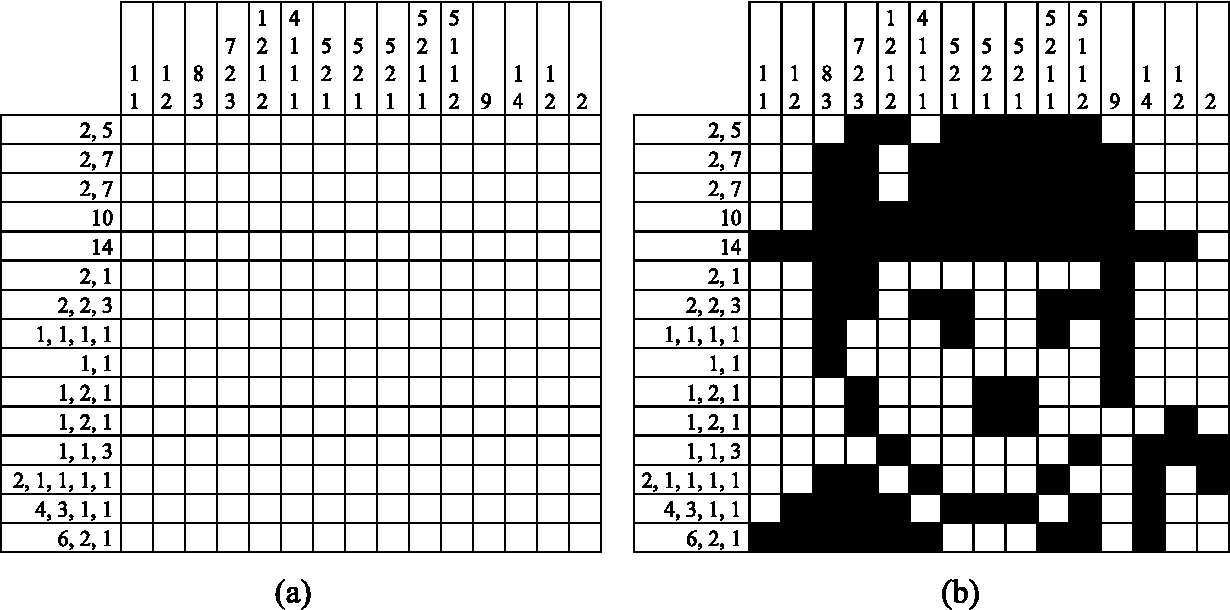
\includegraphics[ width=8cm]{figures/chaplin}
\end{center}

- Rompecabezas de origen japonés
- También conocidos como *griddlers*, *picross*, *paint-by-numbers*
- Compuestos por una matriz de *X* e *Y* número de filas y columnas

\end{frame}

### Motivación

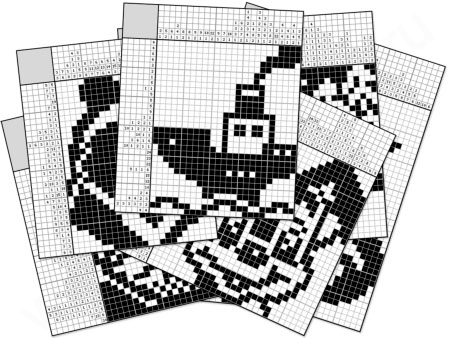
\includegraphics[ width=5cm]{figures/nonogrampromobw}\hspace*{0.5cm}~ 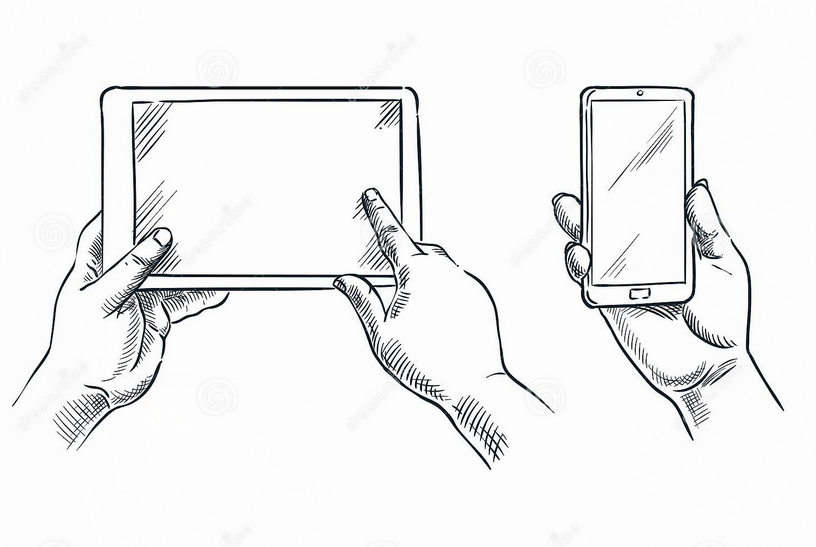
\includegraphics[width=6cm]{figures/smartphones}

- Adaptación de los nonogramas a medios digitales
- Gran potencial creativo
- Crecimiento exponencial de las aplicaciones multiplataforma
- Comunidad más extensa

\end{frame}

### Objetivos

- Plasmar el mundo de los nonogramas en un aplicativo móvil
    - *Android*
    - *iOS*
- Ofecer un *MVP* con el que:
    - Resolver nonogramas
    - Crear niveles y compartirlos \textit{en red}
- Objetivos personales
    - Estudiar el desarrollo de \textit{apps móviles}
    - Comprender la lógica  detrás de los rompecabezas

\end{frame}

# Estudio estratégico

### Estudio estratégico

\begin{center}
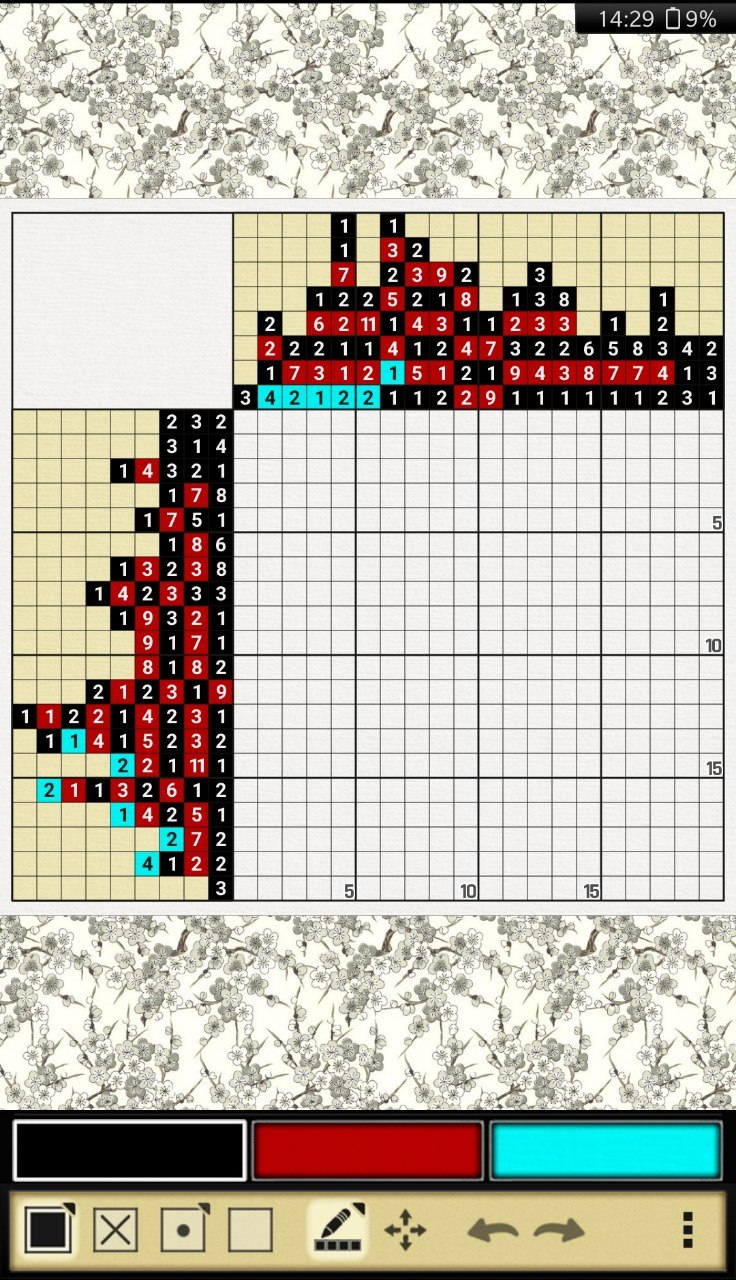
\includegraphics[ width=2.2cm]{figures/nonokatana3}
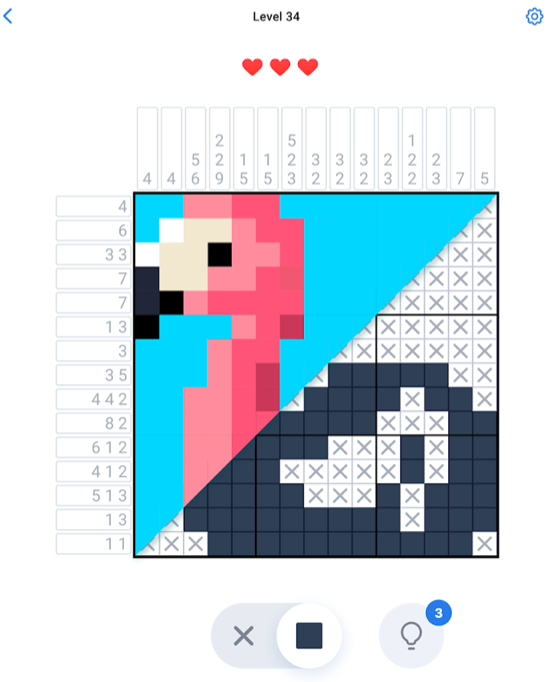
\includegraphics[ width=3cm]{figures/picturecross1}
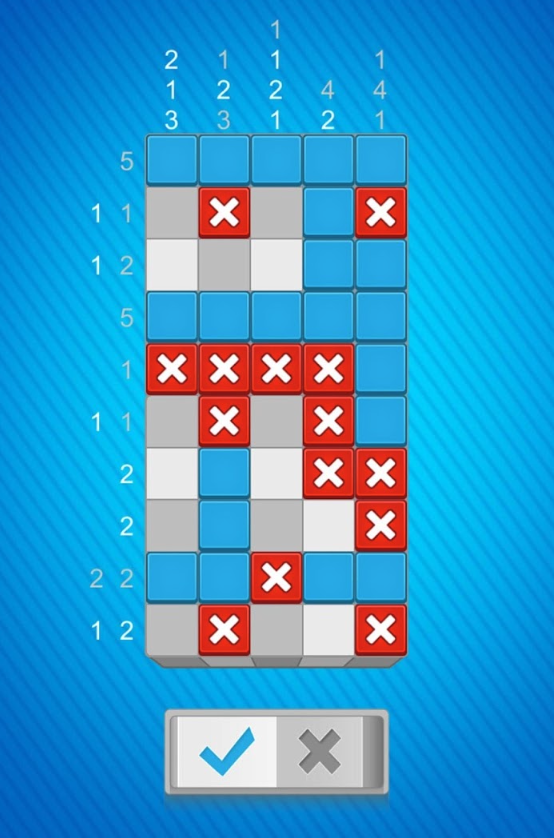
\includegraphics[ width=2.5cm]{figures/infinite2}
\end{center}

- Muy visuales
- Se centran en la experiencia de juego
- Publicidad muy intrusiva

\end{frame}

### Aplicación propuesta

#### Características fundamentales

- Aplicación multiplataforma (\textit{Android} e \textit{iOS})
- Resolución, creación y publicación de nonogramas
- Otras funcionalidades extraídas:
    - Temática especial
    - Multiidioma
    - Autoguardado
    - Servicios in-cloud


---

\end{frame}

# Metodología

### Metodología PXP

\begin{center}
    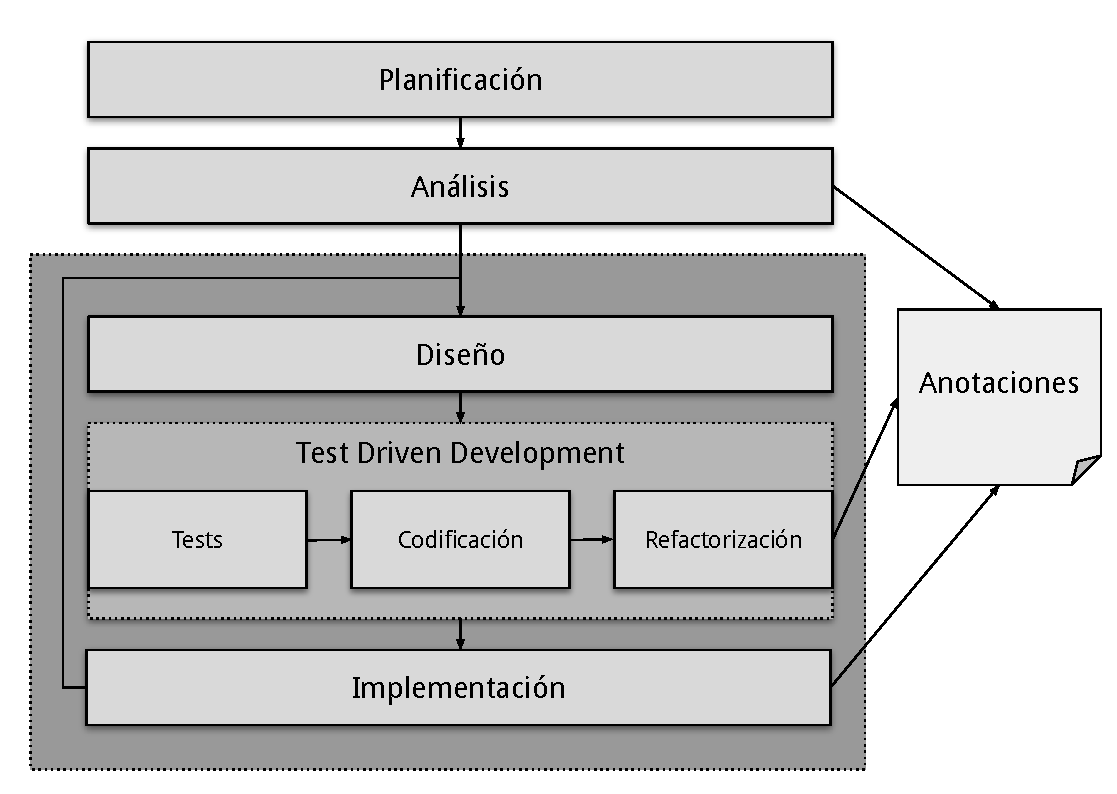
\includegraphics[ width=6cm]{figures/pxpdiagram}
\end{center}

- \textit{Personal Extreme Programming}, subrama de \textit{XP}
- Flujo de las fases similar a \textit{PSP}
- Incorporación de la metodología \textit{TDD}
- Iteraciones mediante retrospectivas

\end{frame}

# Análisis y Diseño 

### Análisis y diseño

\begin{center}
    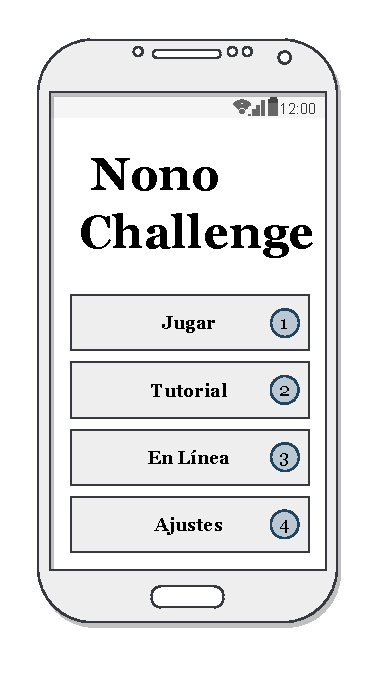
\includegraphics[ width=2.5cm]{figures/screen1}
    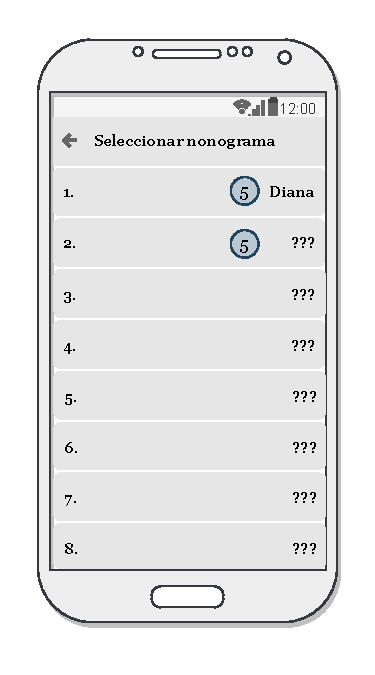
\includegraphics[ width=2.5cm]{figures/screen2}
    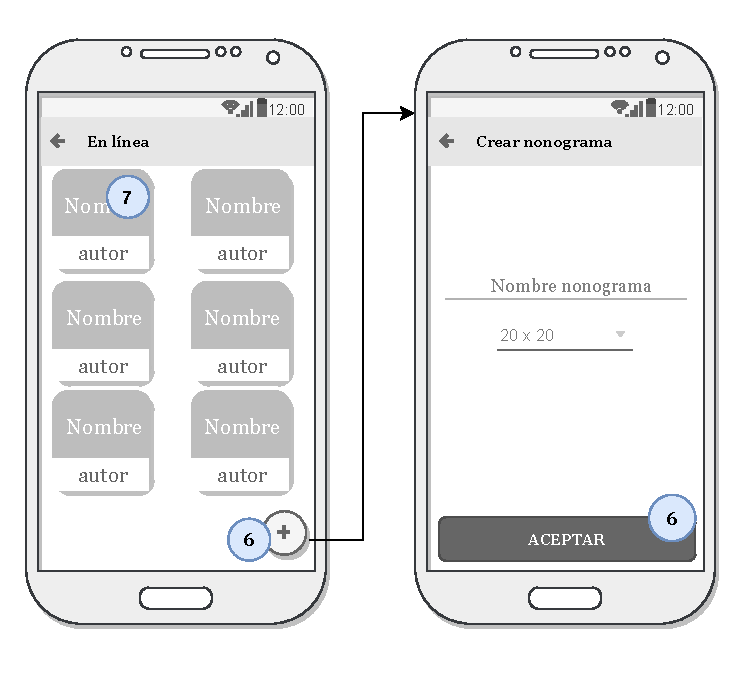
\includegraphics[ width=5cm]{figures/screen3}
\end{center}

- Estandar ISO *IEEE Std 830-1998*
- Requisitos representados en *Mock-ups*


\end{frame}

### Análisis y diseño

\begin{center}
    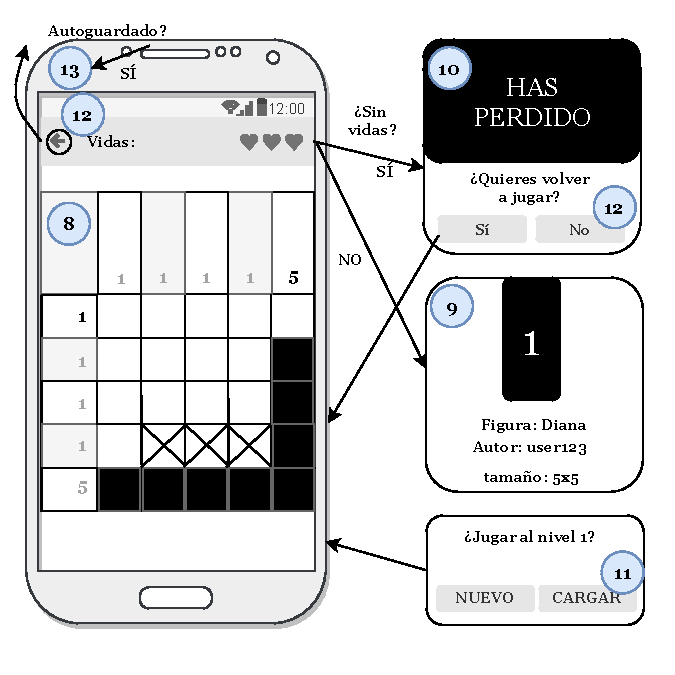
\includegraphics[ width=4.3cm]{figures/screen4}
    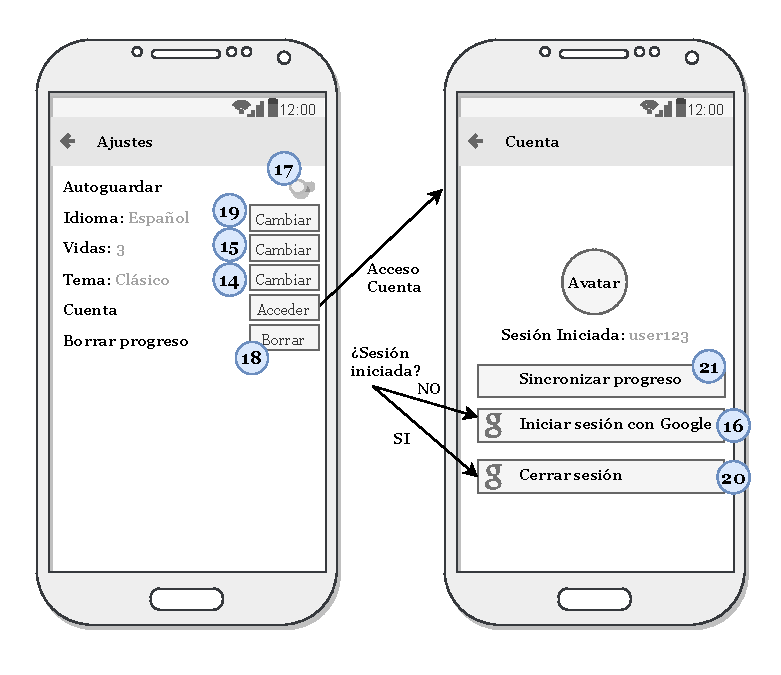
\includegraphics[ width=5cm]{figures/screen5}
\end{center}

#### Resultado

- Componentes comunes
- Simplicidad, reusabilidad y experiencia de uso

---


\end{frame}

# Implementación

### Tecnologías y herramientas

- Aplicativo móvil


\includegraphics[ width=4.3cm]{figures/flutteranddart}

- Autenticación, sincronización en nube y base de datos *realtime*

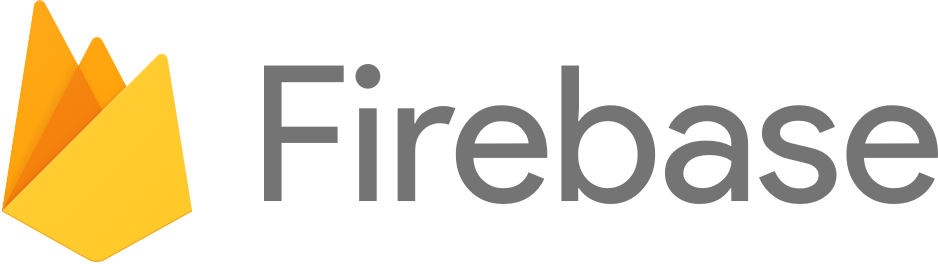
\includegraphics[ width=2.8cm]{figures/firebase}

- Control de versiones e Integración Continua


\includegraphics[ width=1.8cm]{figures/giticon}
\hspace*{0.3cm}~

\includegraphics[ width=2.1cm]{figures/gitlab}


\end{frame}

### Clean Architecture

\begin{center}
   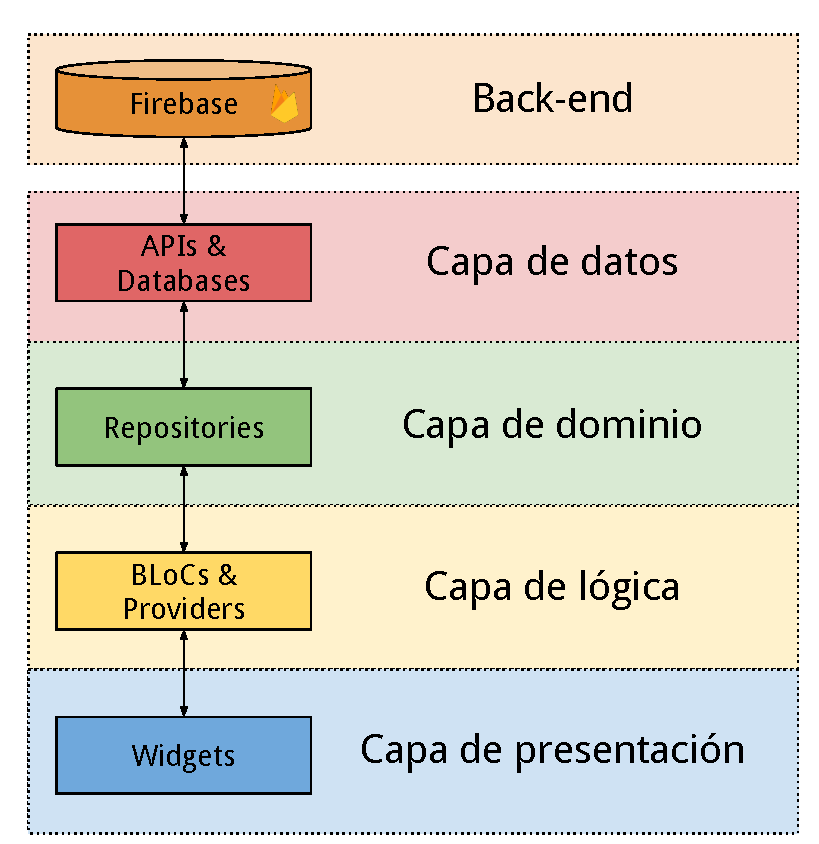
\includegraphics[ width=4cm]{figures/architecture} 
\end{center}

- Arquitectura hexagonal
- Mayor abstracción, modularidad y reusabilidad
- Filosofía de *features*


\end{frame}

### Manejador de estados

\begin{center}
   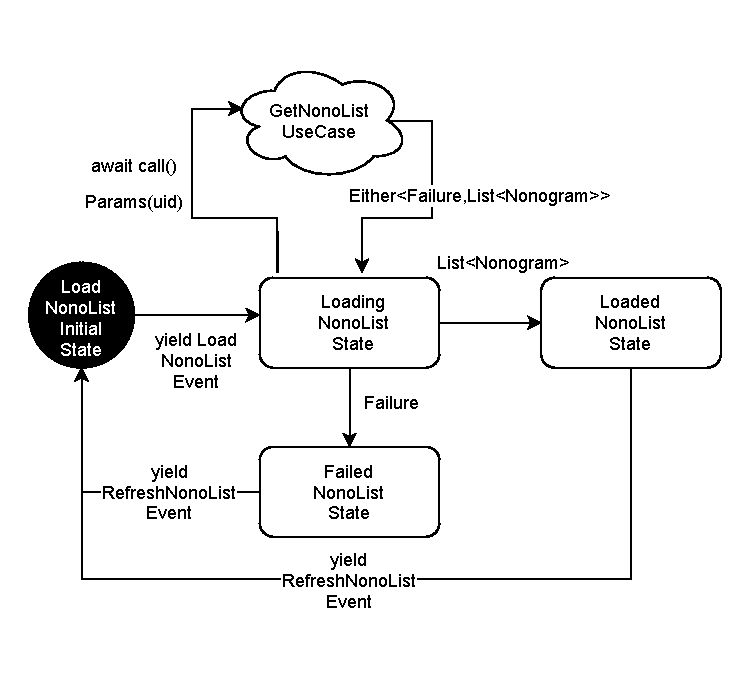
\includegraphics[ width=6cm]{figures/statesNonoList} 
\end{center}

- Patrón *BLoC* y *Provider*
- Flujo de eventos y estados

\end{frame}

# Pruebas

### Pruebas

\begin{center}
   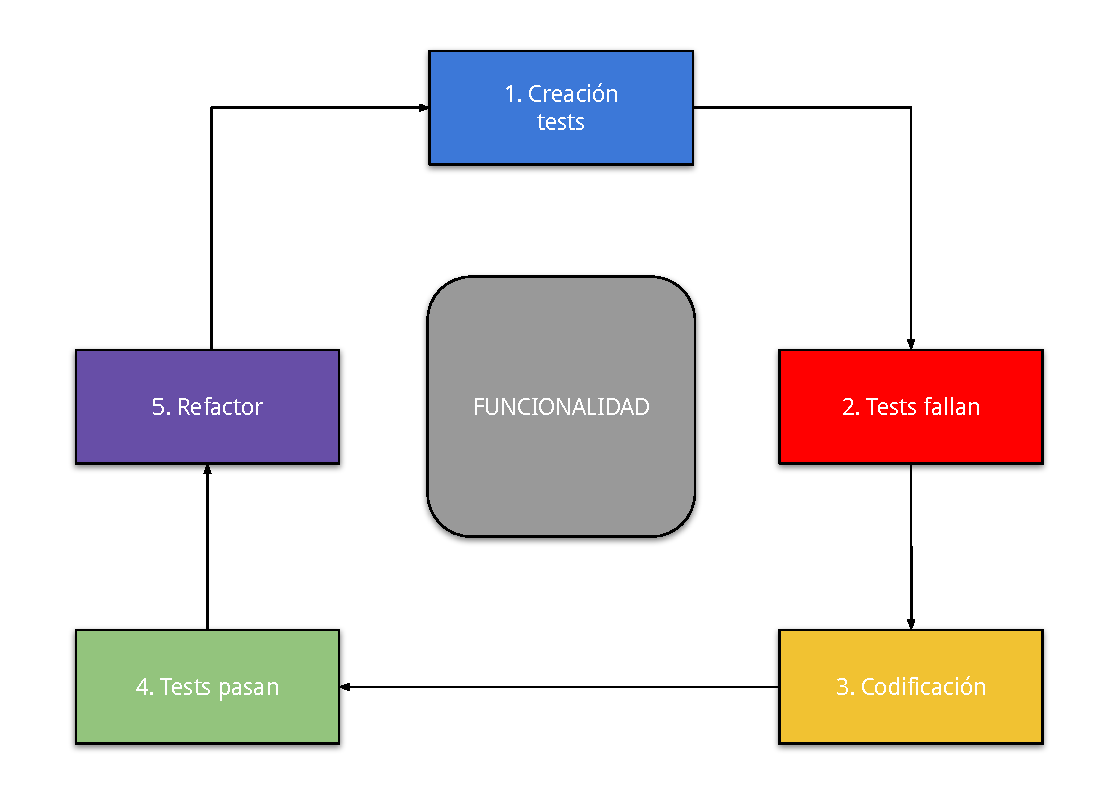
\includegraphics[ width=7cm]{figures/tdddiagram} 
\end{center}

#### Test-Driven-Development (*TDD*)

- Ayuda a comprender la problemática central
- Anticipación a fallos, código más limpio y seguro

---

\end{frame}

# Demo

%%%%%%%%%%%%%%%%%%%%%%

### Demo de NonoChallenge

| Dispositivo | Tipo | SO | Dimen. |
|------:|:-----|---------|:------:| 
|  OnePlus 5T   | Físico |  Android 10  |  6 inch    |  
| IPhone 12 mini   | Emulador | iOS 14.6 |   5'4 inch  | 

  : Características de los dispositivos empleados

\end{frame}

# Trabajo futuro

### Trabajo futuro

- A partir de *Flutter 2.0*
    - Monetización (*Google Mobile Ads*)
    - Adaptación a entornos *web* (*Flutter web*)
    - Adaptación a entornos *desktop* (*Windows*,*MacOs* y *Linux*)
- Inclusión de elementos más visuales
  
\end{frame}

%%novalidate
\end{markdown}


\end{document}
